\section{استخراج قسمت‌های حاوی اطلاعات از اسلاید}\label{subsec:استخراج قسمت‌های حاوی اطلاعات از اسلاید}

اسلاید‌هایی که متخصصان از آن برای تشخیص استفاده می‌کنند، ابعاد بزرگی در حد چند‌ده‌هزار پیکسل را دارند، به طوری که به هیچ‌وجه در
حافظه پردازنده‌های رایج جای نمی‌گیرد.
برای حل این مشکل در این پروژه سعی بر این شد که اسلاید‌ها به تیکه‌های کوچک تر
$512\times512$
 عکس شکسته شوند به طوری که قابل پردازش باشند.
 برای پوشش سلول‌هایی که در ناحیه‌های مرزی عکس و به صورت ناقص قرار می‌گیرند، ناحیه‌‌ها همپوشانی $10$ درصد را با یکدیگر دارند.
یکی از موضوعات مهمی که باید در نظر گرفت، ناحیه‌های غیر مهم و فاقد اطلاعات است که باید در این فرآیند حذف گردند. این کار به دو دلیل انجام می‌شود.
اولا اینکه این قسمت‌ها، بخش بزرگی از اسلاید‌ها را تشکیل می‌دهند و با حذف این موارد می‌توان در استفاده از منابع پردازشی صرفه جویی کرد
و دوما اگر تعداد زیادی از عکس‌هایی که هنگام آموزش مدل استفاده می‌کنیم، از این نوع باشند، دقت مدل کاهش پیدا می‌کند و مدل در فرآیند یادگیری با مشکل مواجه می‌شود.
دلیل این امر هم این است که این عکس‌ها حاوی ویژگی‌های مورد نظر ما برای تشخیص سلول‌های سرطانی نیستند و مدل در حین فرآیند آموزش، ویژگی‌های نامربوطی را از روی این عکس‌ها یاد می‌گیرد.

برای حل این موضوع، روشی که به‌کار گرفته شد، استفاده از واریانیس لاپلاسین ناحیه است.
لاپلاسین یک عکس از محاسبه مشتق دوم روی شدت رنگ‌های پیکسل‌های آن محاسبه می‌شود
و در نتیجه لبه و گوشه‌های عکس مقدار بیشتری می‌گیرد.
برای محاسبه مشتق دوم برای یک عکس از رابطه \ref{eqn:derivitive_of_image} استفاده شده است که در آن $Im(x)$ مقدار شدت رنگ را در موقعیت x از تصویر نشان می‌دهد.
\begin{equation}
	\label{eqn:derivitive_of_image}
		\begin{split}
			   & Im'(x) = Im(x+1) - Im(x), Im'(x+1) = Im(x+2) - Im(x+1)\\
			   & Im"(x) = Im(x+2) - 2 \times Im(x+1) + Im(x)
		\end{split}
\end{equation}

بعد از محاسبه واریانس شدت رنگ پیکسل‌ها در لاپلاسین عکس و استفاده از یک آستانه عکس‌هایی که مقدار کمتری دارند فیلتر می‌شوند.
به این ترتیب ناحیه‌های فاقد اطلاعات که مقدار لاپلاسین کمی نیز دارند حذف می‌شوند.

برای بدست آوردن مقدار بهینه آستانه و همچنین آزمودن این روش، به ترتیب زیر عمل شده است.
\begin{enumerate}
    \item ابتدا حدس اولیه 500 برای آستانه انتخاب شد و اسلاید‌ها با توجه به این آستانه به قطعه‌های کوچک عکس در آمدند.
    مقدا اولیه آستانه در این مرحله، نیاز به دقت بالایی ندارد، زیرا همانطور که در قسمت بعد نیز توضیح داده خواهد شد، از آن برای انتخاب اسلاید‌ها استفاده می‌کنیم.
    این حدس اولیه نیز با مشاهده مقادیر به صورت عملی و از روی نواحی چند اسلاید انتخاب شد.
    توزیع تعداد و درصد قطعه عکس‌های مجموع اسلایدها در تصویر ~\ref{fig:patch_distribution_with_initial_and_final_threshold} آمده است.
    \begin{figure}
        \begin{center}
            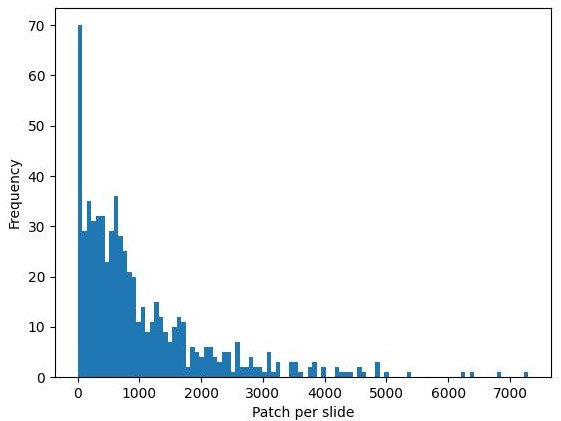
\includegraphics[width=0.48\linewidth]{figs/introduction/subs/challenges/patch_distribution_old_500_threshold.jpeg}
            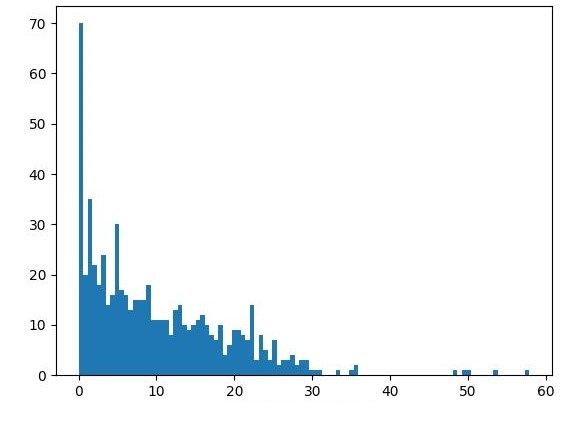
\includegraphics[width=0.48\linewidth]{figs/introduction/subs/challenges/patch_percent_distribution_old_threshold_500.jpeg}
            \hspace{.2cm}
            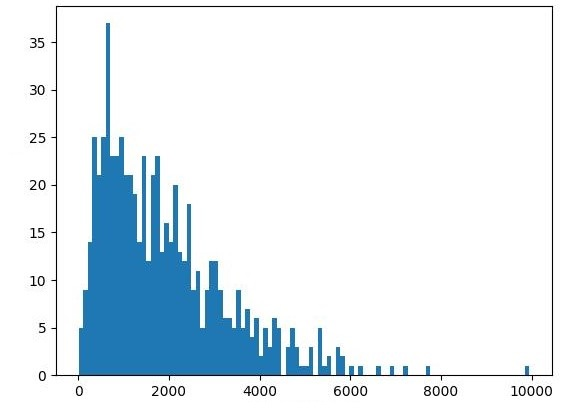
\includegraphics[width=0.48\linewidth]{figs/introduction/subs/challenges/patch_distribution_new_298_threshold.jpeg}
            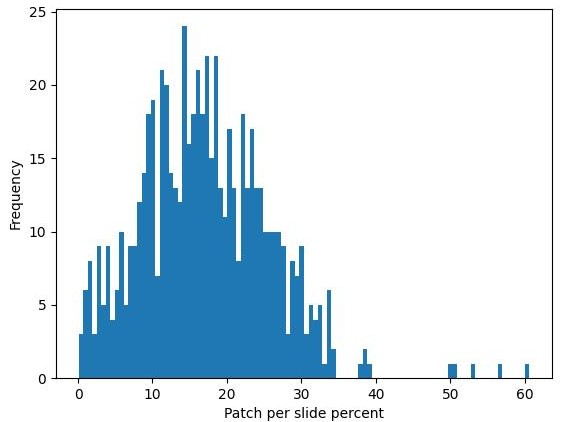
\includegraphics[width=0.48\linewidth]{figs/introduction/subs/challenges/patch_percent_distribution_new_threshold_298.jpeg}
        \end{center}
    	
        \caption[نمودارهای توزیع تعداد قطعه عکس‌های تولید شده و درصد قطعه عکس‌های تولید‌شده نسبت به تعداد کل]{
        	        	نمودار‌ها به ترتیب از راست به چپ توزیع تعداد قطعه عکس‌های تولید‌شده از هر اسلاید و درصد قطعه عکس‌های تولید‌شده نسبت به تعداد کل را برای هر اسلاید به ازای آستانه اولیه $500$ و آستانه نهایی بدست آمده $298$ در قسمت پایانی را نشان می‌دهد.}
        \label{fig:patch_distribution_with_initial_and_final_threshold}
    \end{figure}
    \item سپس سه اسلاید از پایین بازه و سه اسلاید از بالای بازه مشخص‌شده در نمودار توزیع قطعه عکس‌ها انتخاب شدند.
    سه اسلاید بالای بازه اسلاید‌هایی هستند که روش به‌کار رفته تعداد زیادی قطعه عکس از آن‌ها تولید کرده است و سه اسلاید پایین بازه اسلاید‌هایی هستند که به دلیل نابهینه بودن آستانه، قطعه عکس‌های کمی را برای آن‌ها تولید کرده است.
    \item برای شش اسلاید انتخاب شده، به صورت دستی و با استفاده از نرم افزار \cite{gimp}\lr{GIMP} ماسک‌هایی تولید شد.
    \item در قدم بعد، باید معیار‌هایی را برای روش به‌کار رفته انتخاب کرد تا با استفاده از آن‌ها بتوان آستانه بهینه را پیدا کرد و در نهایت آن را ارزیابی کرد.
    همانطور که در قسمت‌های قبل گفته شد، فیلتر ناحیه‌های فاقد اطلاعات، اهمیت زیادی برای ما دارد از این رو، در ارزیابی این روش علاوه بر دقت\LTRfootnote{Accuracy}، صحت\LTRfootnote{Precision} نیز عامل مهمی در کارکرد درست است.
    صحت، با توجه به فرمول \ref{eqn:precision_and_description} هرچه به مقدار عددی 1 نزدیک تر باشد به این معناست که ناحیه‌های بدست آمده از این روش، به احتمال بالاتری دارای اطلاعات هستند و در نتیجه ناحیه‌های فاقد اطلاعات کمتری تولید می‌شوند.
	\begin{equation}
		\label{eqn:precision_and_description}
		\begin{split}
		   	&Precision = \frac{TP}{TP + FP}\\
			&TruePositive(TP) :\textit{روش به درستی عکس را غیر پس زمینه تشخیص داده}\\
			&TrueNegative(TN) :\textit{ روش به درستی عکس را پس زمینه تشخیص داده}\\
			&FalsePositive(FP) :\textit{ روش اشتباهاً عکس را غیر پس زمینه تشخیص داده}\\
			&FalseNegative(FN) :\textit{ روش اشتباهاً عکس را پس زمینه تشخیص داده}
		\end{split}
	\end{equation}
    دقت روش نیز با توجه به رابطه \ref{eqn:accuracy} محاسبه می‌شود.
   	\begin{equation}
    	\label{eqn:accuracy}
    	\begin{split}
    		&Accuracy = \frac{TP + TN}{TP + FP + TN + FN}\\
    	\end{split}
    \end{equation}
    
    \item حال با توجه به این دو معیار، قطعه کدی نوشته شد که شش اسلاید و ماسک‌های مربوط به آن‌ها را به عنوان ورودی می‌گیرد و با شروع از آستانه 500 و محاسبه ماتریس درهم ریختگی\LTRfootnote{Confusion Matrix}، در جهتی آستانه را تغییر می‌دهد تا دو معیار گفته‌شده بیشینه شوند.
    لازم به ذکر است، در نهایت از تابع هدف\LTRfootnote{Objective Function}
     $0.25\times\text{Precision}+0.75\times\text{Accuracy}$
      برای یافتن آستانه استفاده شد تا صحت مقدار پایینی به خود نگیرد.
    در هر دوره از اجرای کد، از هر اسلاید 2000 (با توجه به اینکه درصد زیادی از اسلاید‌ها را پس‌زمینه تشکیل می‌دهد، عدد بزرگی انتخاب شد تا آستانه در هر دور، در جهت درستی حرکت کند) و در مجموع
     $2000 \times 6$ 
     قطعه عکس مورد بررسی قرار می‌گیرد به صورتی که آستانه در جهت افزایش تابع هدف و با اندازه پرش\LTRfootnote{Jump Size} $120$ و نرخ نزولی\LTRfootnote{Decay Rate} $0.85$، کاهش و یا افزایش پیدا می‌کند.
    نمودار تغییرات تابع هدف و آستانه در طی اجرای برنامه در تصویر ~\ref{fig:objective_function_and_threshold_changes} آمده است که در آن‌ها تابع هدف و آستانه به ترتیب به مقادیر $0.96$ و $298$ همگرا شده‌اند.
    \begin{figure}
        \begin{center}
            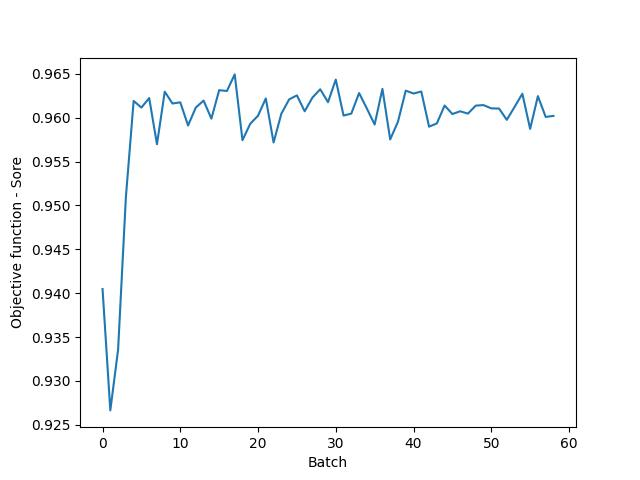
\includegraphics[width=0.48\linewidth]{figs/introduction/subs/challenges/laplacian_threshold_score_history_chart.jpeg}
            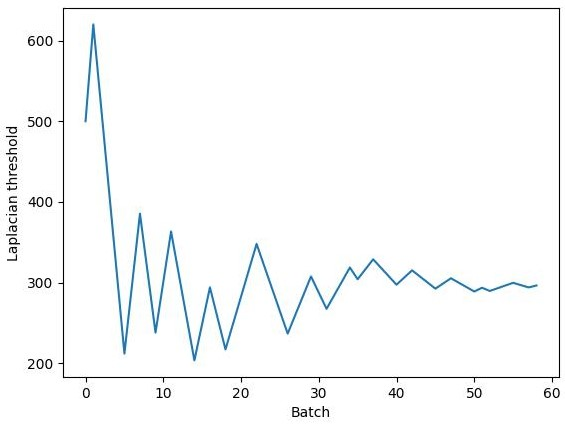
\includegraphics[width=0.48\linewidth]{figs/introduction/subs/challenges/laplacian_threshold_history_chart.jpeg}
        \end{center}
        \caption[تغیرات تابع هدف و آستانه برای فیلتر عکس‌های فاقد اطلاعات]
        {به ترتیب از راست به چپ، تغیرات تابع هدف و آستانه قابل مشاهده است که در نهایت تابع هدف به مقدار $0.96$ و آستانه به $298$ همگرا شده است.}
        \label{fig:objective_function_and_threshold_changes}
    \end{figure}
    اسلاید‌ها و ماسک‌های به‌کار رفته آن‌ها در تصویر~\ref{fig:threshold_train_slides_and_menuall_masks} ارائه شده است و دقت و حساسیت روش بر روی این شش اسلاید نیز در جدول~\ref{table:laplacian_acc_details} آمده است.
    \begin{table}[t]
        \centering
        \begin{latin}
            \begin{tabular}{|c|c|c|c|c|}
                \hline
                \rl{اسلاید} & \rl{{ماتریس درهم ریختگی}} & \rl{دقت} & \rl{صحت}
                \\
                \hline
                \hline
                \text{1} & \lr{TP: $4624$  FP: $126$ TN: $14100$ FN: $226$} & $0.98$ & $0.97$\\
                \text{2} & \lr{TP: $1103$  FP: $172$ TN: $3758$  FN: $7$} & $0.96$ & $0.86$\\
                \text{3} & \lr{TP: $7615$  FP: $92$  TN: $20871$ FN: $234$} & $0.98$ & $0.98$\\
                \text{4} & \lr{TP: $78$    FP: $18$  TN: $1880$  FN: $4$} & $0.98$ & $0.81$\\
                \text{5} & \lr{TP: $1138$  FP: $4$   TN: $6671$  FN: $492$} & $0.94$ & $0.99$\\
                \text{6} & \lr{TP: $460$   FP: $0$   TN: $19618$ FN: $1426$} & $0.93$ & $0.99$\\
                \hline
                \text{In Total} & \text{TP: $15018$ FP: $412$ TN: $66898$ FN: $2389$} & $0.96$ & $0.97$\\
                \hline
            \end{tabular}
        \end{latin}
        \caption[دقت روش لاپلاسین برای تشخیص نواحی پس زمینه از غیر پس زمینه]
        {
        ستون اول این جدول، شماره اسلاید را مشخص می‌کند.
        در ستون دوم ماتریس درهم ریختگی روش لاپلاسین بر روی اسلاید آن آمده است.
        ستون و چهارم به ترتیب دقت و صحت روش ذکر شده برای فیلتر کردن نواحی فاقد اطلاعات را نشان می‌دهد.
    }
        \label{table:laplacian_acc_details}
    \end{table}

    \begin{figure}
        \begin{center}
            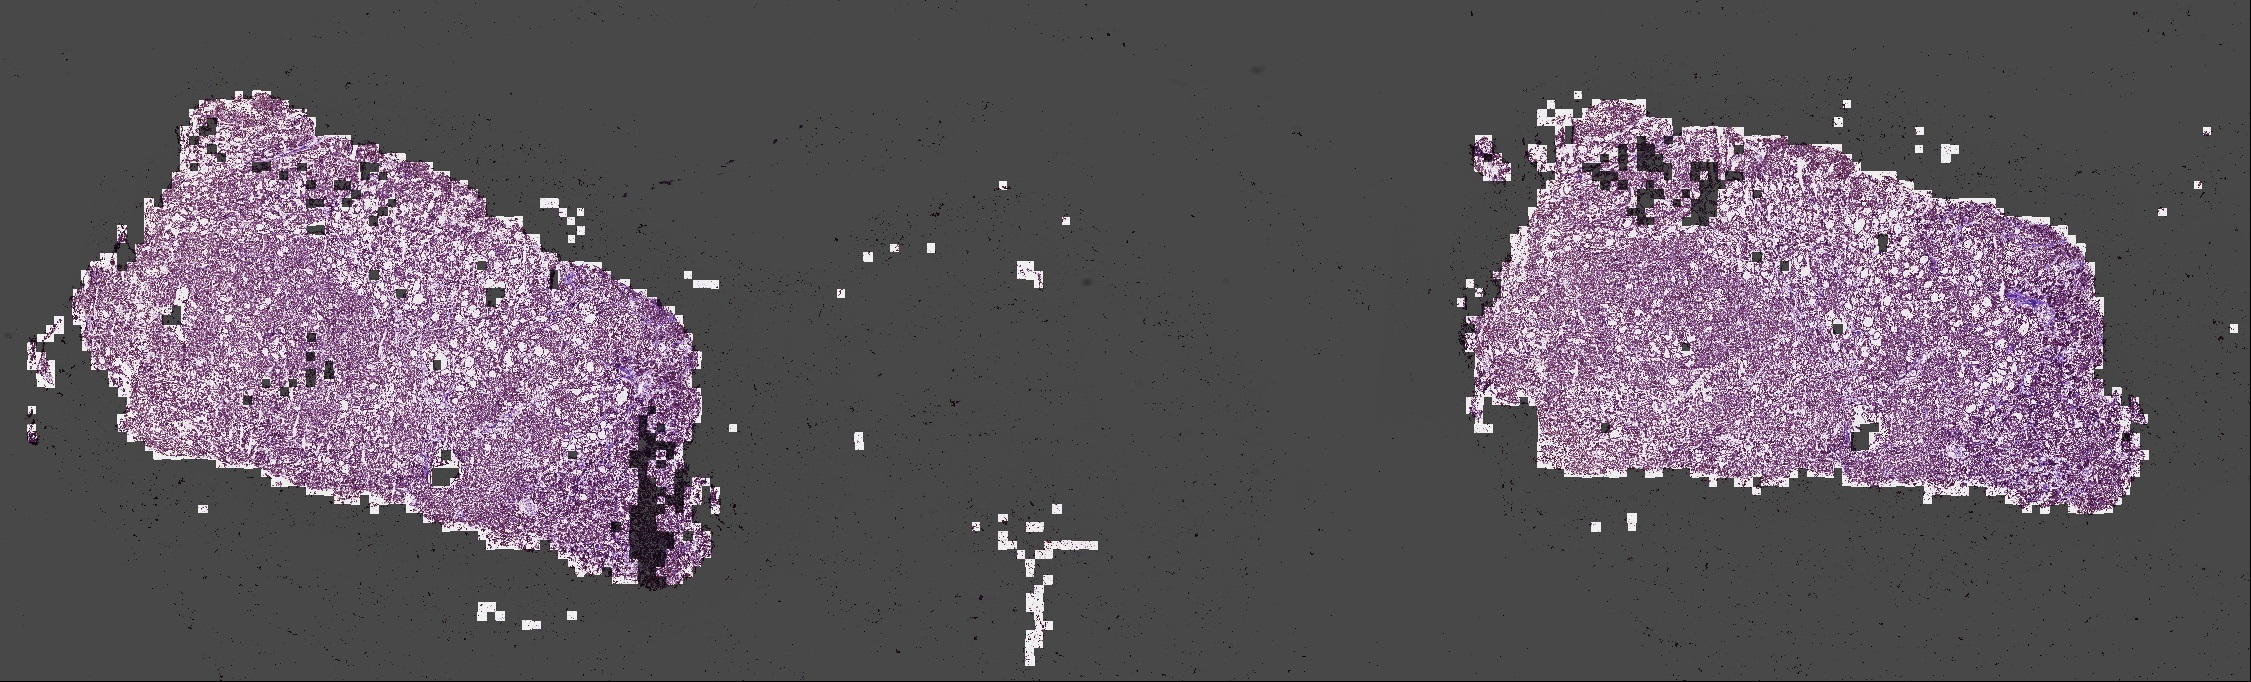
\includegraphics[width=0.48\linewidth]{figs/introduction/subs/challenges/evaluate_slides/TCGA-DJ-A1QG-01A-01-TSA.04c62c21-dd45-49ea-a74f-53822defe097__2000_generated_mask.jpg}
            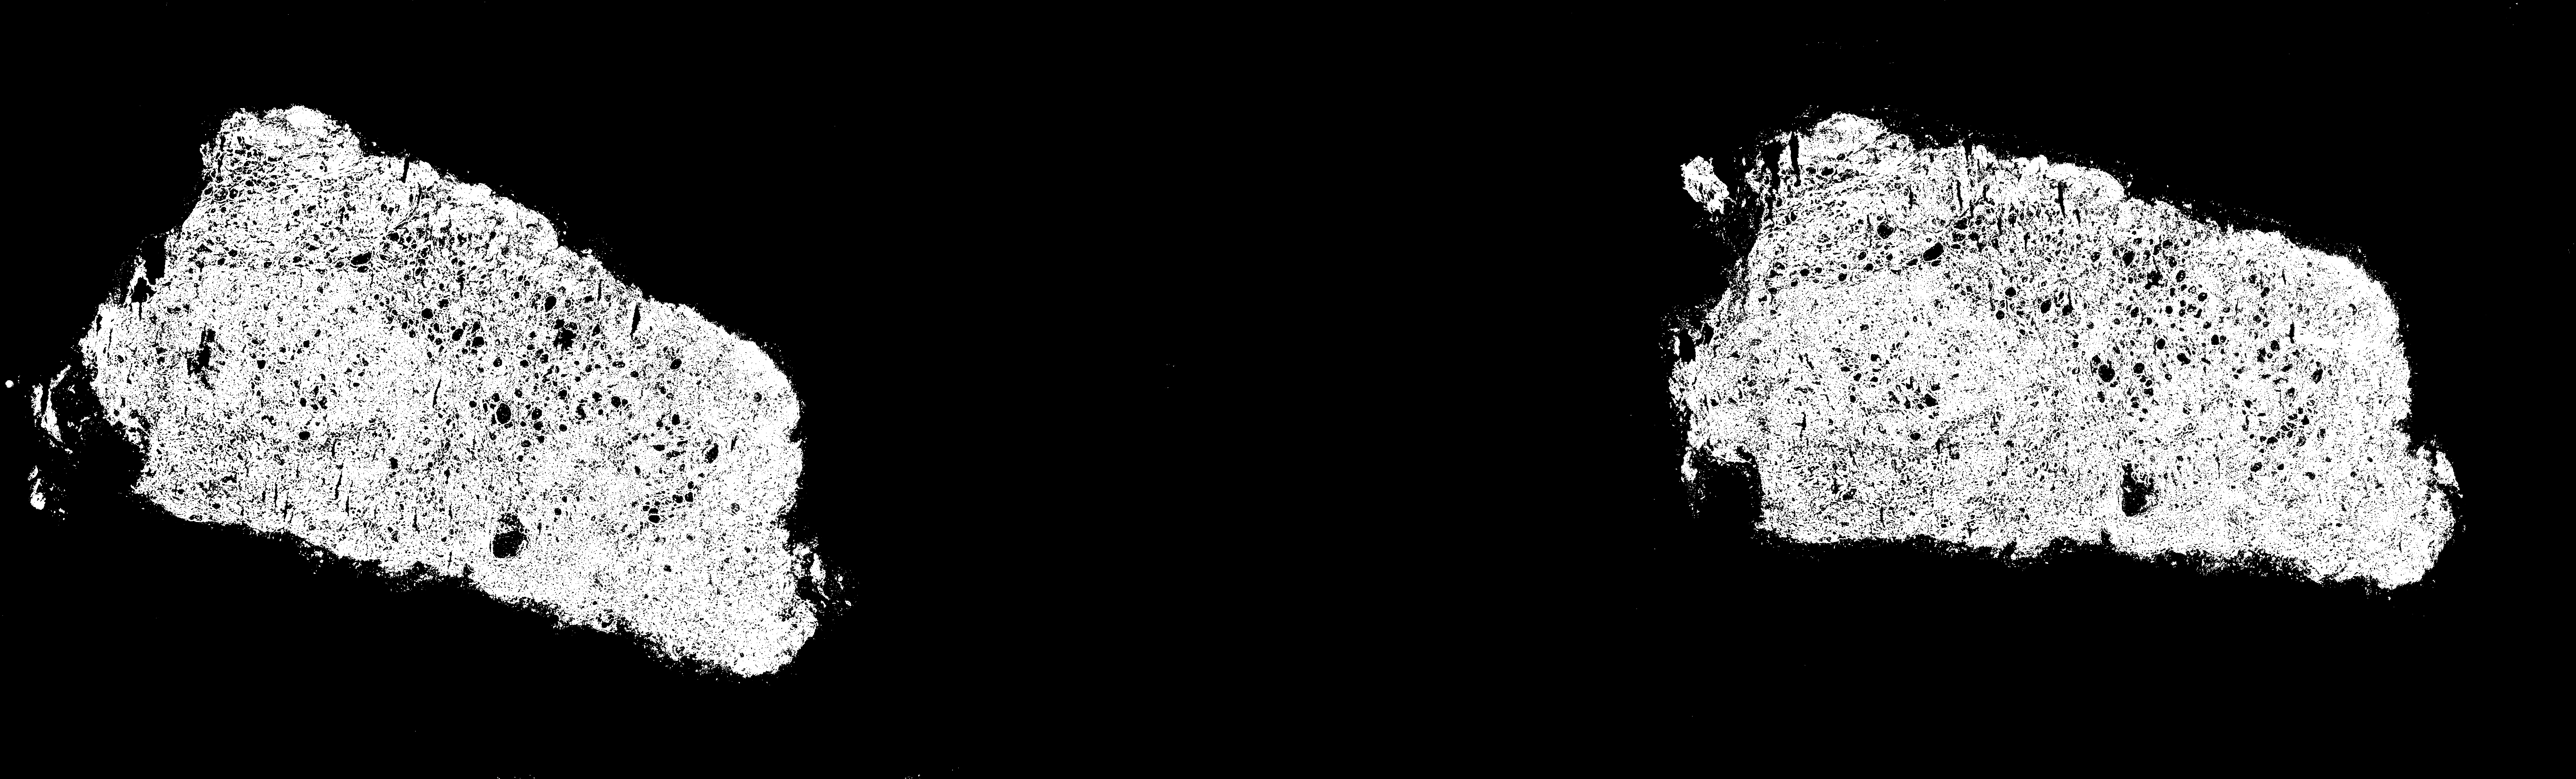
\includegraphics[width=0.48\linewidth]{figs/introduction/subs/challenges/evaluate_slides/TCGA-DJ-A1QG-01A-01-TSA.04c62c21-dd45-49ea-a74f-53822defe097__2000_masked.png}
            \hspace{.2cm}
            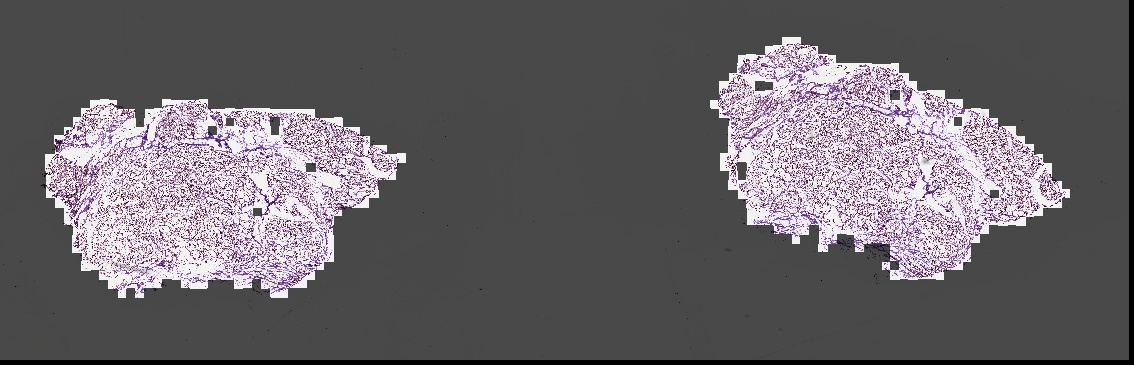
\includegraphics[width=0.48\linewidth]{figs/introduction/subs/challenges/evaluate_slides/TCGA-EL-A3TB-11A-01-TS1.6E0966C9-1552-4B30-9008-8ACF737CA8C3__2000_generated_mask.jpg}
            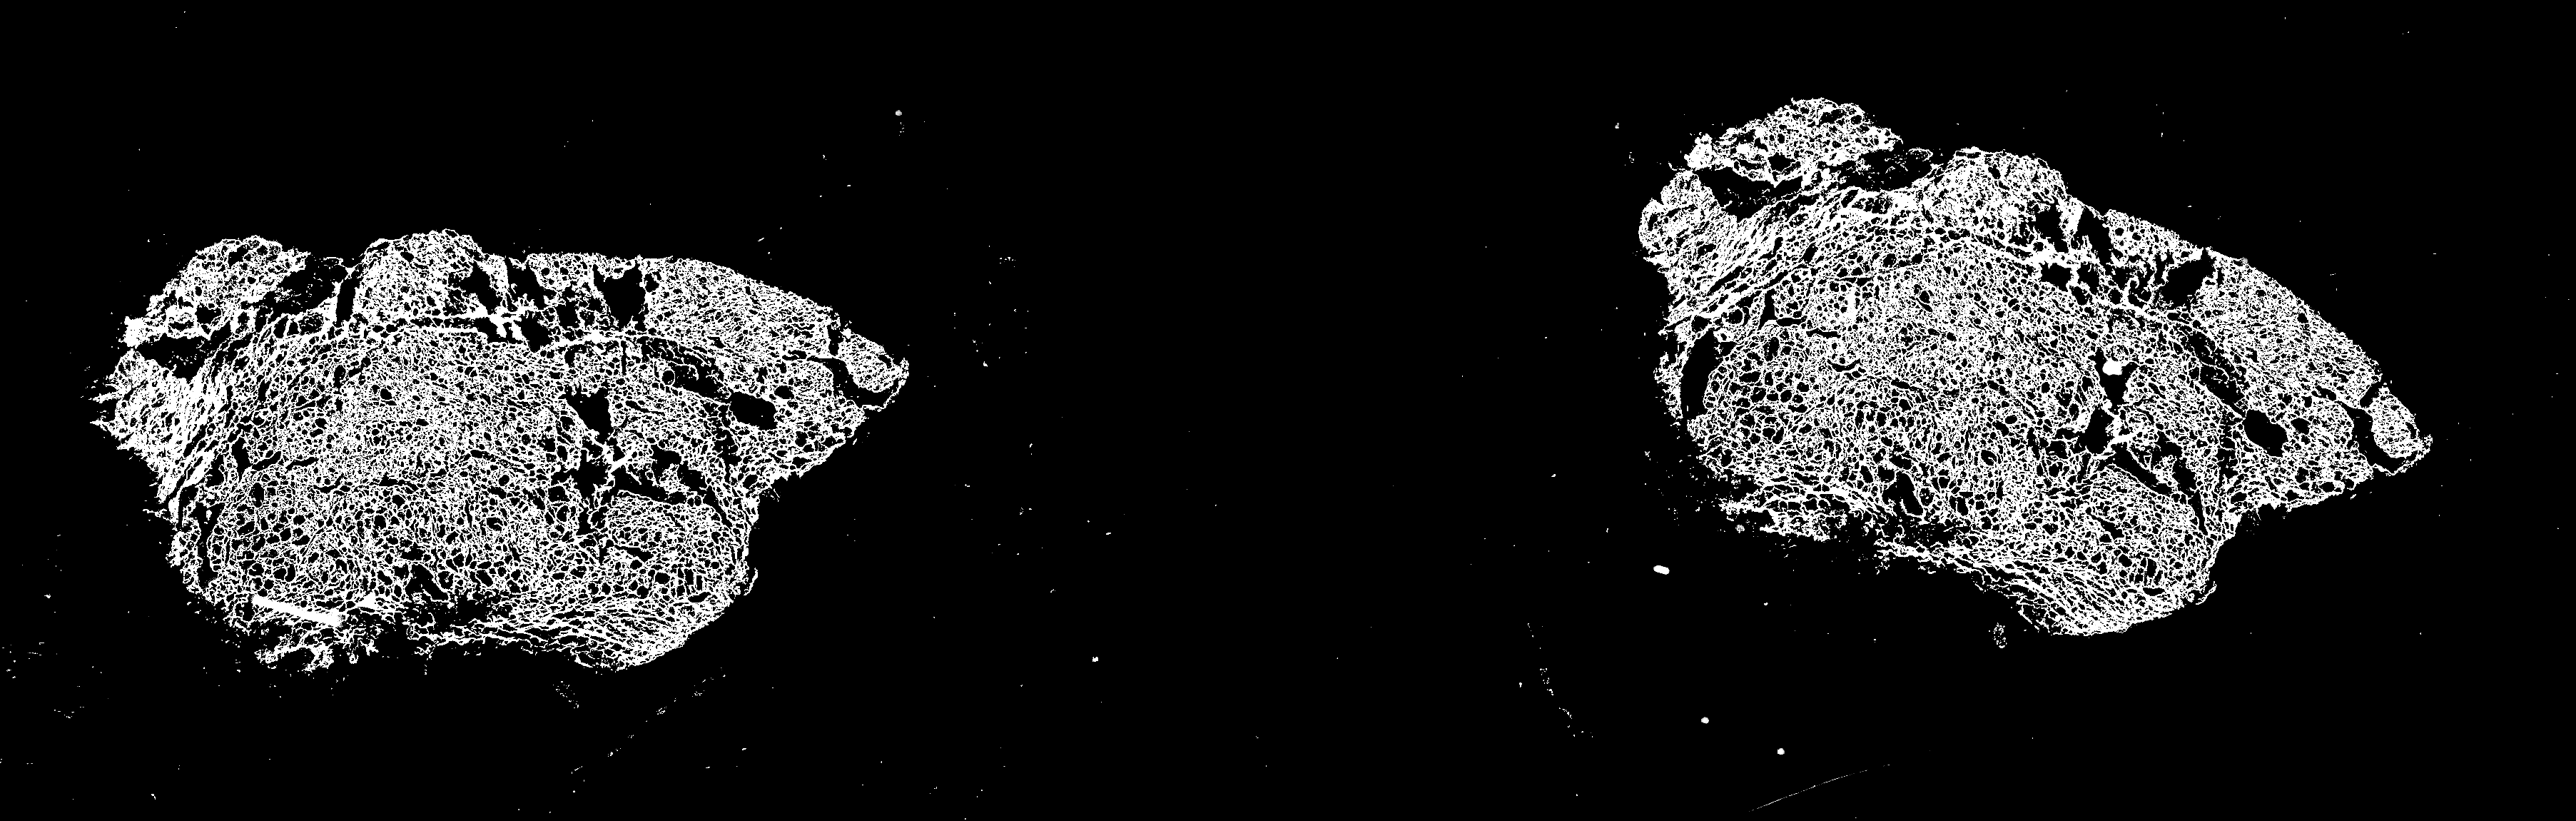
\includegraphics[width=0.48\linewidth]{figs/introduction/subs/challenges/evaluate_slides/TCGA-EL-A3TB-11A-01-TS1.6E0966C9-1552-4B30-9008-8ACF737CA8C3__2000_masked.png}
            \hspace{.2cm}
            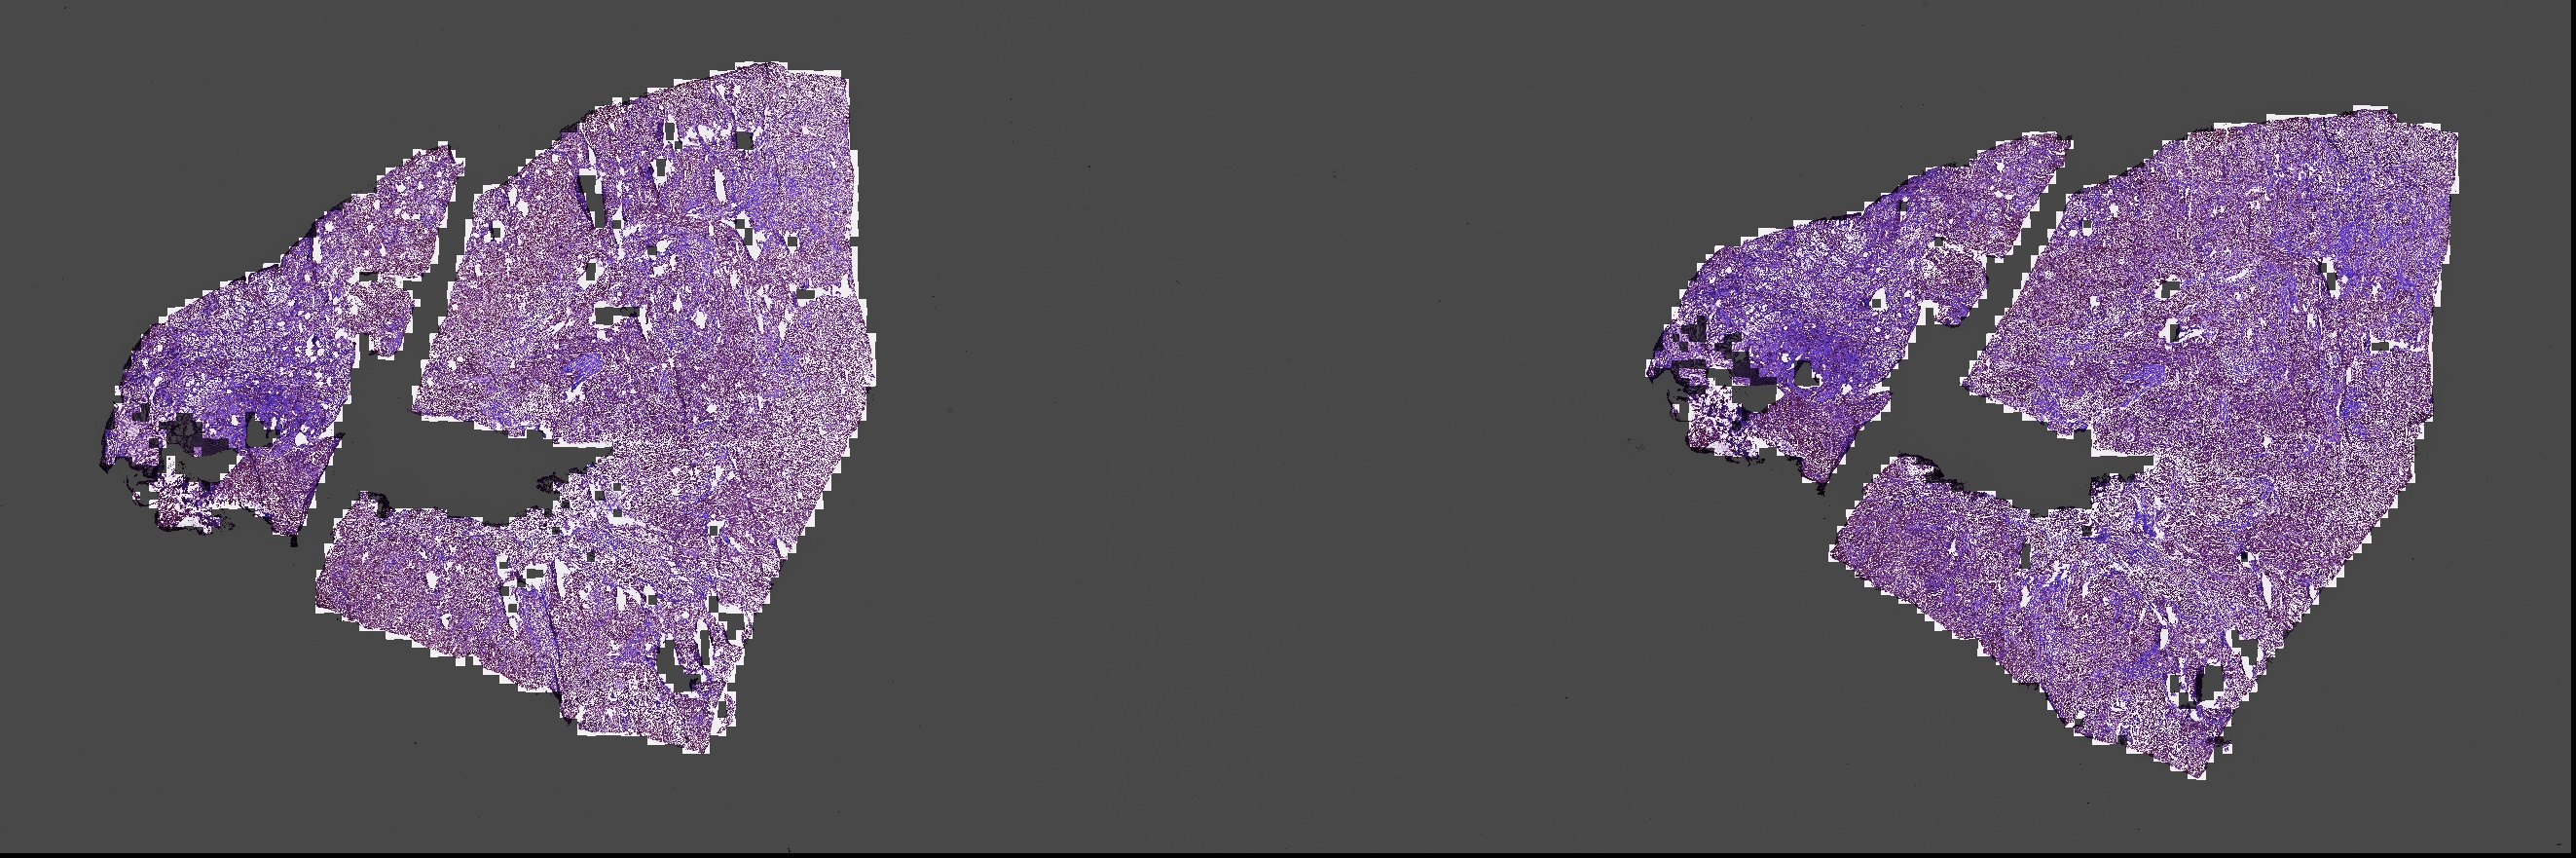
\includegraphics[width=0.48\linewidth]{figs/introduction/subs/challenges/evaluate_slides/TCGA-ET-A39O-01A-01-TSA.3829C900-7597-4EA9-AFC7-AA238221CE69_7000_generated_mask.jpg}
            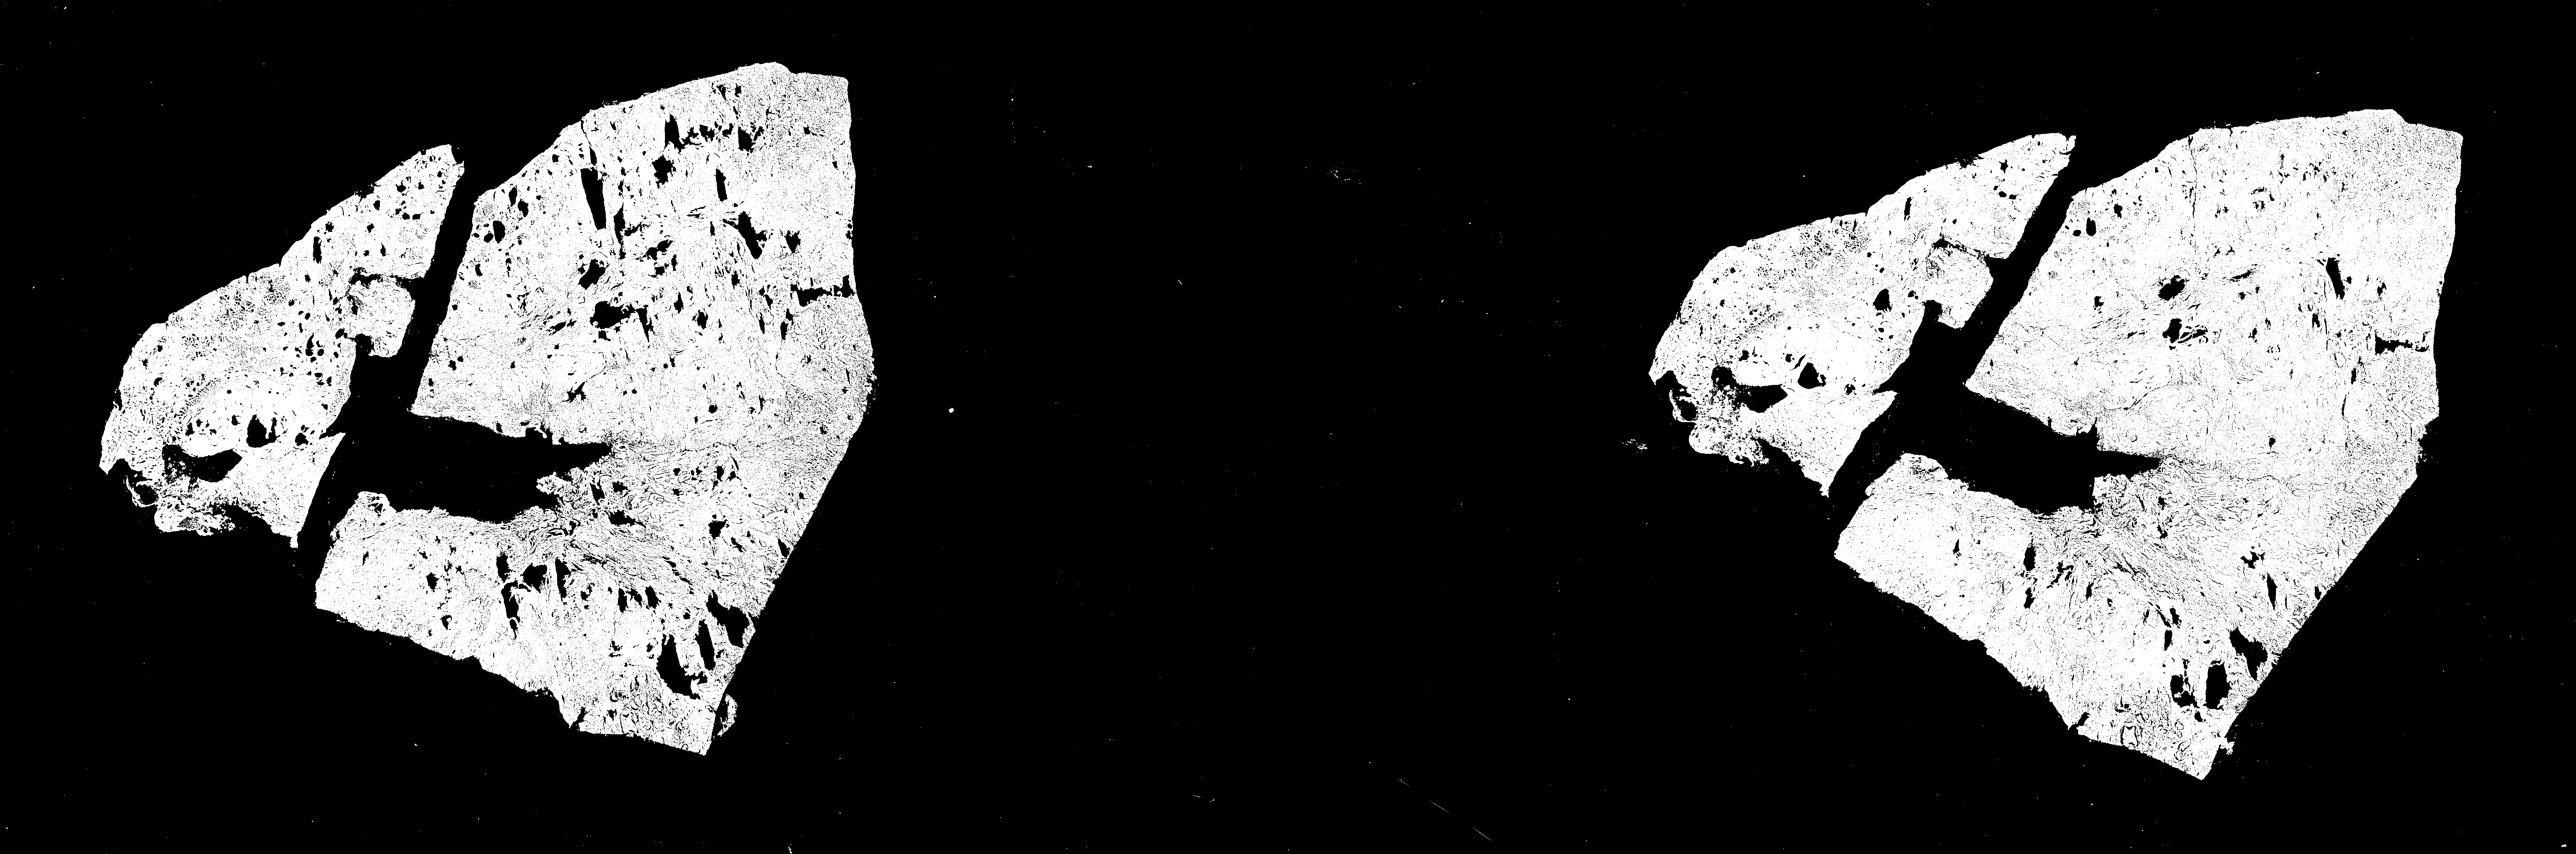
\includegraphics[width=0.48\linewidth]{figs/introduction/subs/challenges/evaluate_slides/TCGA-ET-A39O-01A-01-TSA.3829C900-7597-4EA9-AFC7-AA238221CE69_7000_masked.png}
            \hspace{.2cm}
            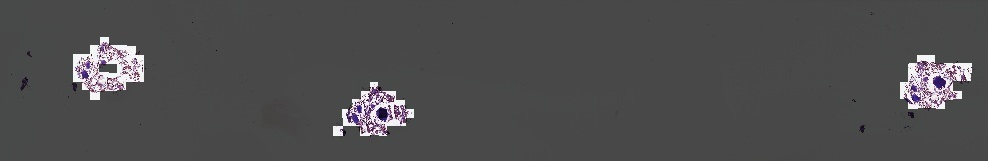
\includegraphics[width=0.48\linewidth]{figs/introduction/subs/challenges/evaluate_slides/TCGA-EL-A4K7-11A-01-TS1.C08B59AA-87DF-4ABB-8B70-25FEF9893C7F__70_generated_mask.jpg}
            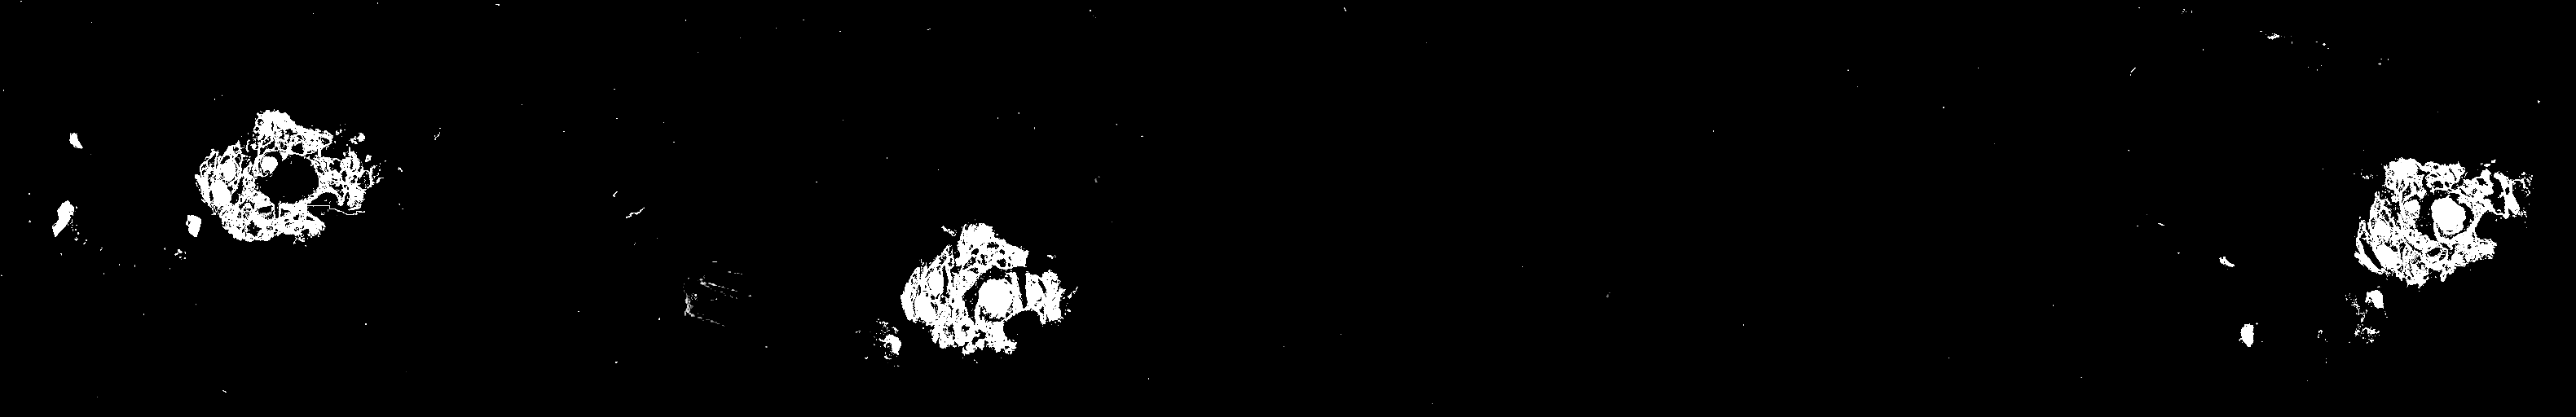
\includegraphics[width=0.48\linewidth]{figs/introduction/subs/challenges/evaluate_slides/TCGA-EL-A4K7-11A-01-TS1.C08B59AA-87DF-4ABB-8B70-25FEF9893C7F__70_masked.png}
            \hspace{.2cm}
            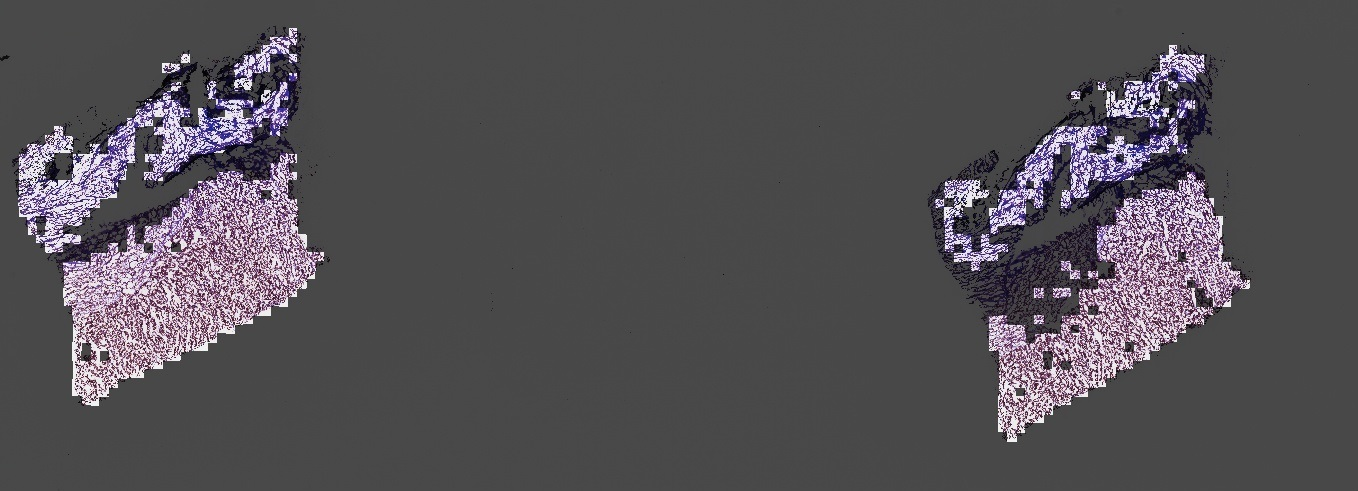
\includegraphics[width=0.48\linewidth]{figs/introduction/subs/challenges/evaluate_slides/TCGA-ET-A39N-01A-01-TSA.C38FCE19-9558-4035-9F0B-AD05B9BE321D___198_generated_mask.jpg}
            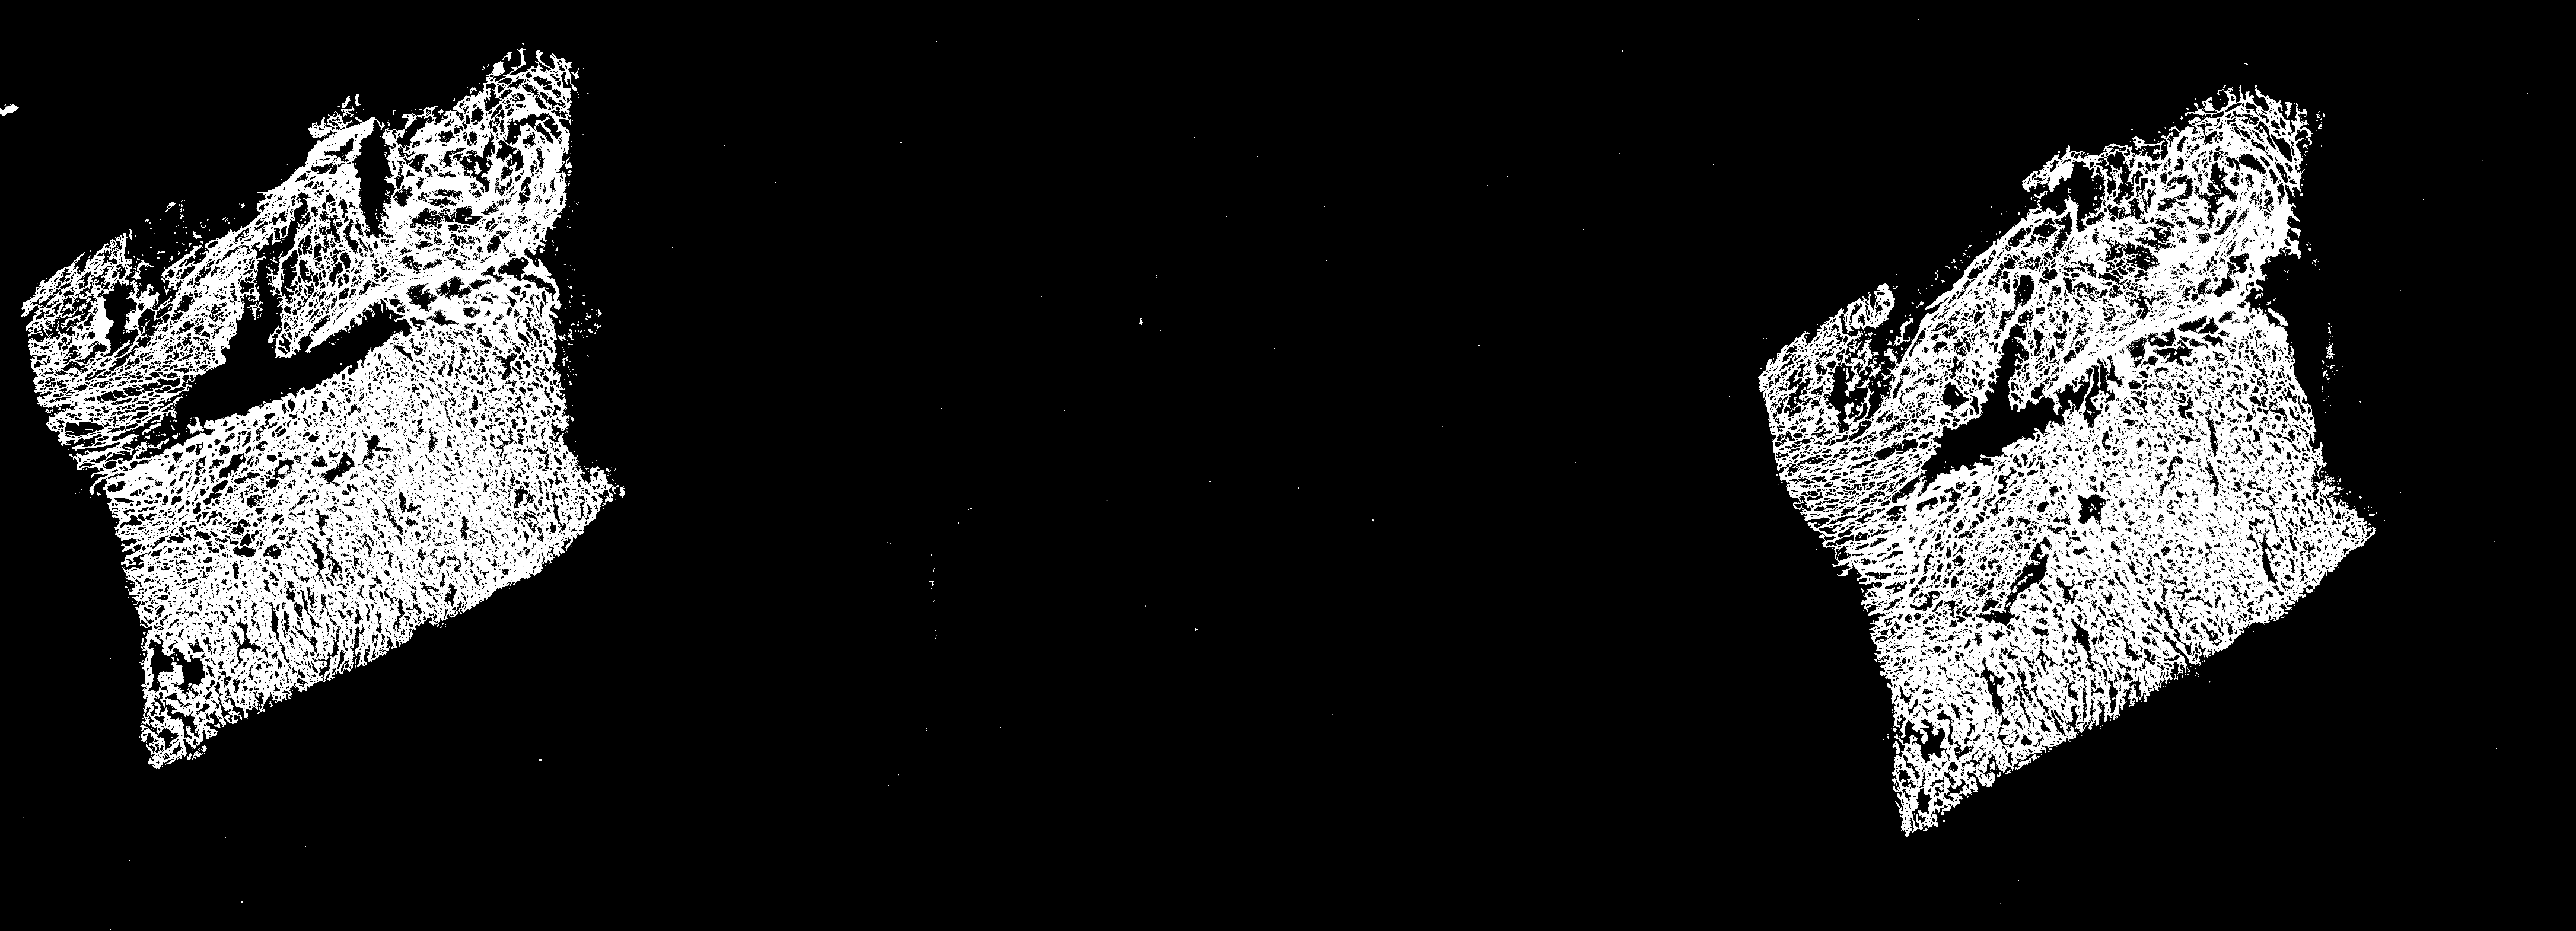
\includegraphics[width=0.48\linewidth]{figs/introduction/subs/challenges/evaluate_slides/TCGA-ET-A39N-01A-01-TSA.C38FCE19-9558-4035-9F0B-AD05B9BE321D___198_masked.png}
            \hspace{.2cm}
            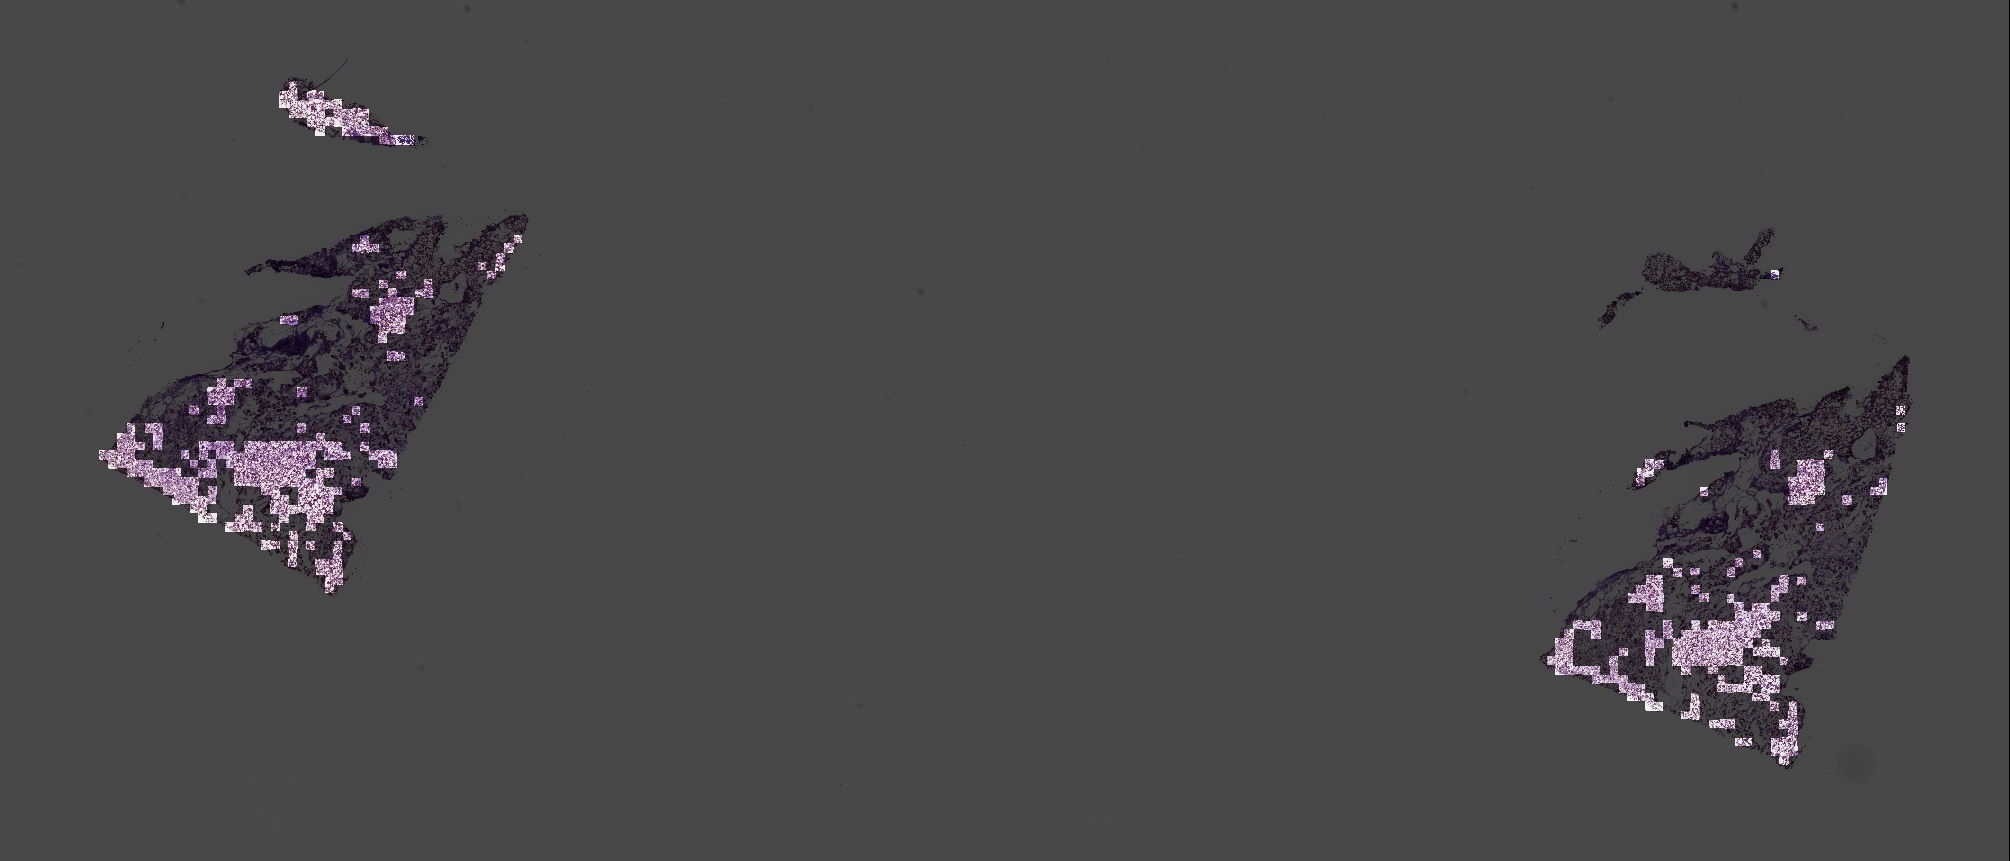
\includegraphics[width=0.48\linewidth]{figs/introduction/subs/challenges/evaluate_slides/TCGA-BJ-A3F0-01A-01-TSA.728CE583-95BE-462B-AFDF-FC0B228DF3DE__3_generated_mask.jpg}
            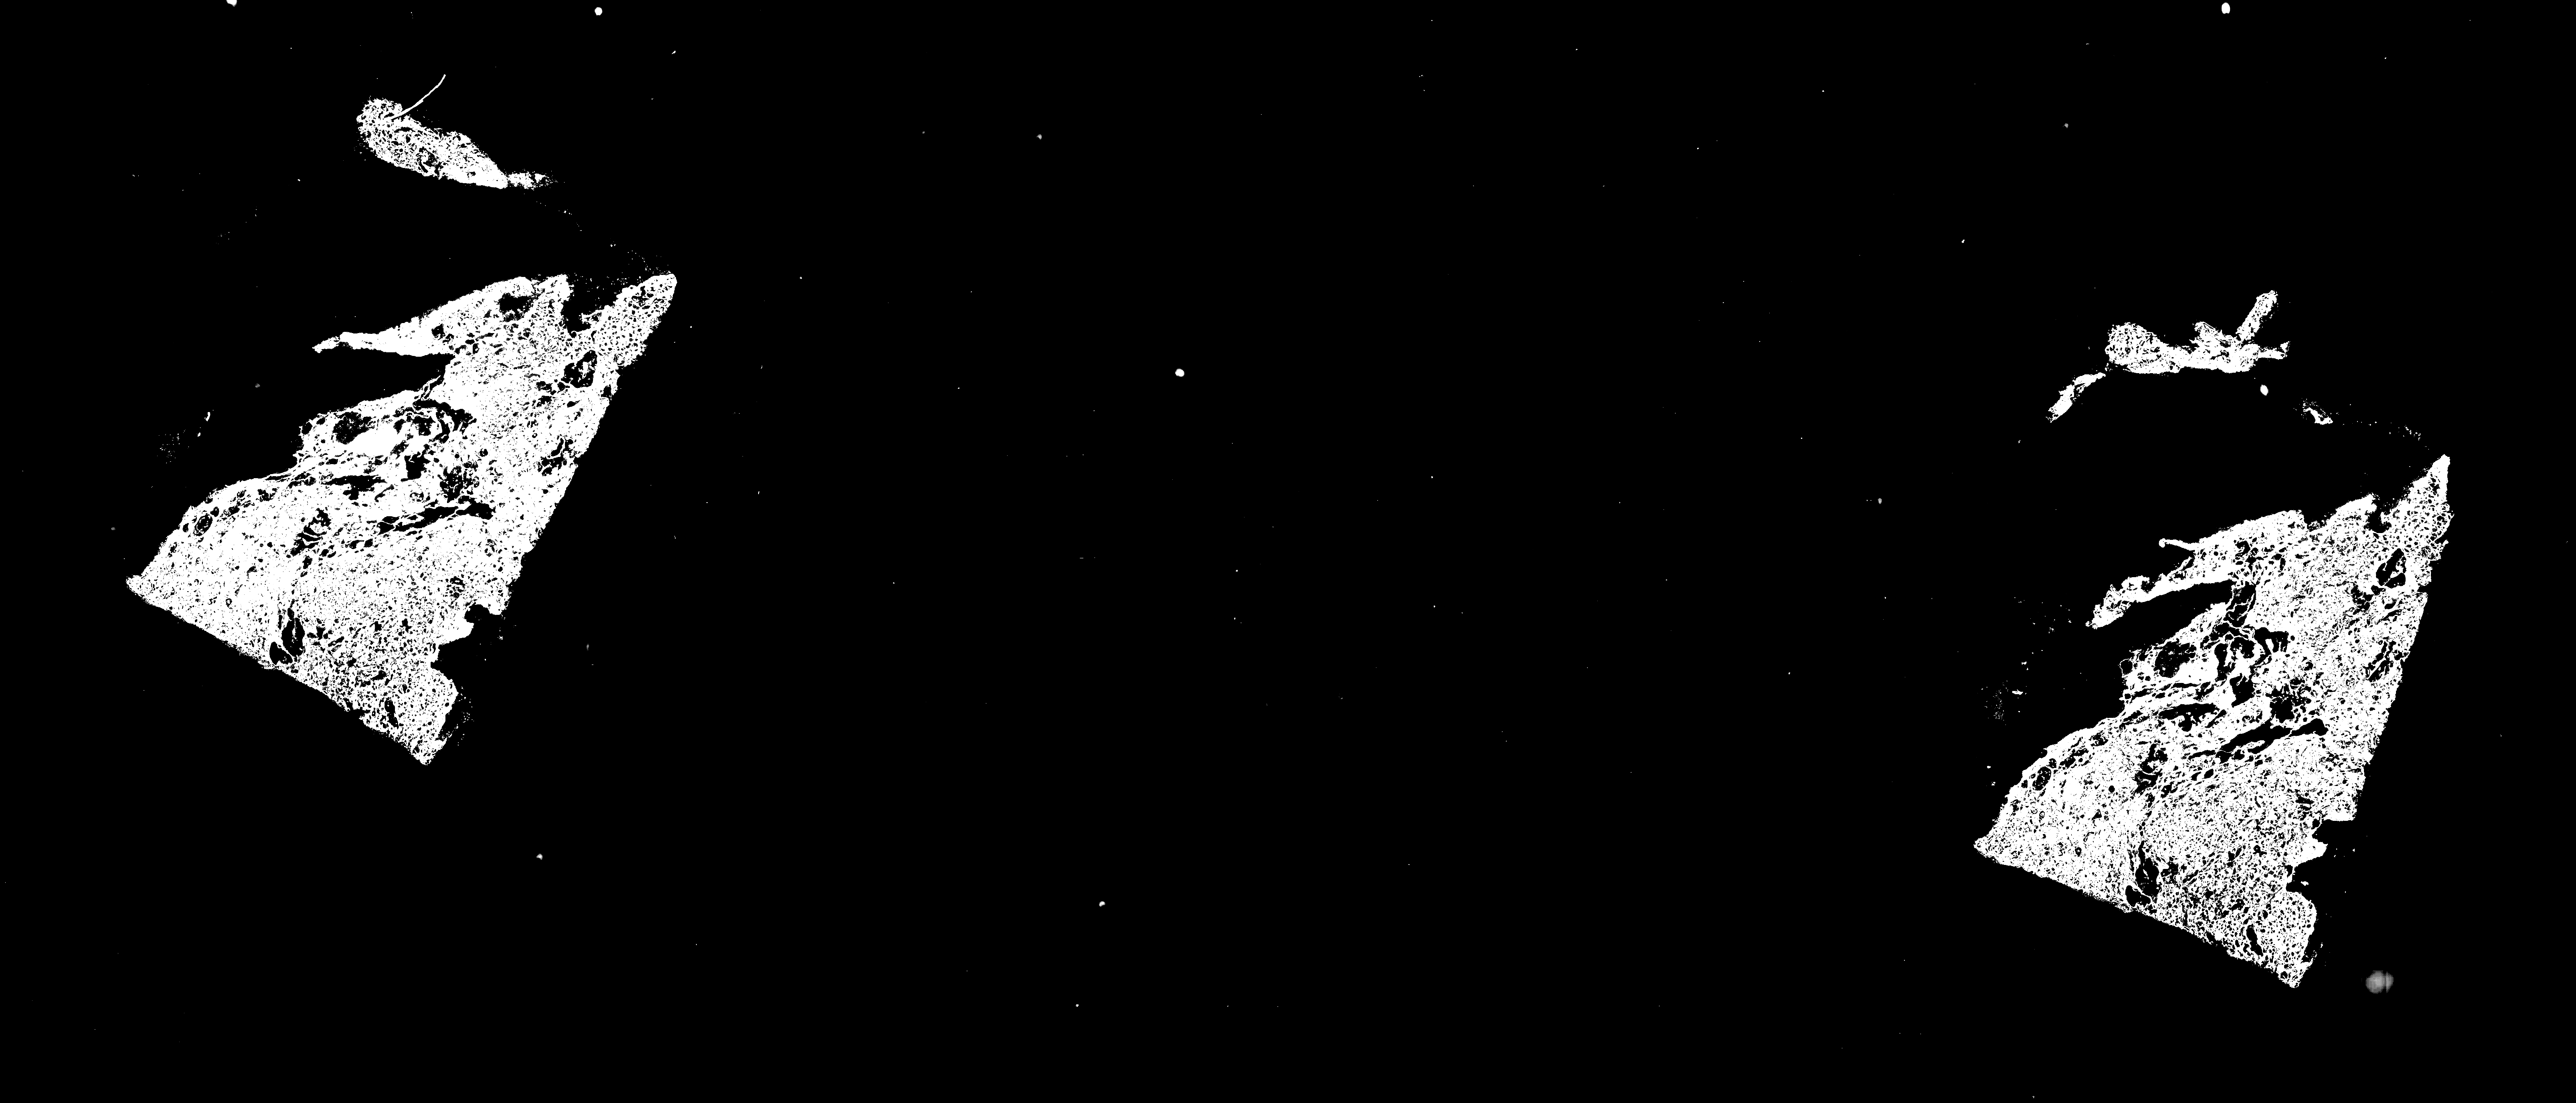
\includegraphics[width=0.48\linewidth]{figs/introduction/subs/challenges/evaluate_slides/TCGA-BJ-A3F0-01A-01-TSA.728CE583-95BE-462B-AFDF-FC0B228DF3DE__3_masked.png}
        \end{center}
        \caption[نواحی استخراج شده و ماسک‌های مرتبط]{ناحیه‌های استخراج‌شده شش اسلاید $1$, $2$, $3$, $4$, $5$, $6$ در آستانه 298 و ماسک‌های مرتبط با آن‌ها}
        \label{fig:threshold_train_slides_and_menuall_masks}
    \end{figure}
\end{enumerate}
بعد از یافتن آستانه، می‌توان اسلاید‌ها را یکی پس از دیگری خواند و نواحی مورد نیاز برای آموزش مدل را استخراج کرد.
با توجه به توضیحات داده‌شده برای این روش استخراج، در ادامه به دو تا از مزیت‌های آن اشاره می‌کنیم:
\begin{itemize}
    \item از آنجایی که حجم داده‌ای که با آن‌ها کار داریم بسیار زیاد است و اسلاید‌های زیادی نیاز به پیش‌پردازش دارند سرعت و دقت عامل مهمی در عملکرد است.
    در این روش، بعد از تهیه ماسک‌ها برای شش اسلاید ذکر‌شده به صورت دستی و تعیین آستانه، دیگر نیاز به دخالت انسان نداریم، از این روی، این روش دقت و سرعت بالایی را داراست.
    \item همانطور که پیشتر نیز گفته شد، فایل‌های دیجیتال اسلاید‌ها، از طریق اسکن نمونه‌ها توسط دستگاه و در زیر میکروسکپ تهیه می‌شوند.
    در بعضی مواقع به دلیل شرایط فیزیکی نمونه، خطای دستگاه و یا حتی خطای انسانی ممکن است نمونه و یا قسمتی از آن به درستی اسکن نشود.
    این نواحی نیز علاوه بر نواحی پس زمینه اطلاعات مورد نیاز ما را ندارند و یا از دست داده‌اند و حالت بلوری به خود گرفته‌اند.
    با توجه به ماهیت روش استخراج ذکر شده، این مشکل در این فرآیند حل می‌شود.
    لاپلاسین یک تصویر حاوی اطلاعاتی نظیر گوشه‌ها و خطوط است از این روی، یکی از روش‌های اصلی تشخیص بلوری بودن تصویر است، زیرا در این تصاویر اطلاعاتی مانند خطوط اندکی محو می‌شوند.
    با توجه به اینکه مبنای اصلی روش استخراج ذکر‌شده نیز لاپلاسین تصویر است، در طی این فرآیند تصاویر بلوری مقدار واریانس لاپلاسین کمتری گرفته و خود به خود حذف می‌گردند.
\end{itemize}
